\section{Лекция 16 от 18.01.2016}
Вспомним предыдущую лекцию и кое-что дополним
\begin{Comment}
\ 
\begin{enumerate}
    \item Элемент $0$ --- единственный.
    \item И элемент $-a$ единственный.
    \item Даже элемент $1$ единственный.
    \item Как это ни удивительно, но $a^{-1}$ тоже единственный.
\end{enumerate}
\end{Comment}
Легко увидеть, что пункты 2 и 4 доказываются одинаково с точностью до замены операции, как и пункты 1 и 3.

\begin{proof}
Докажем пункт 3. Если существует $1'$ --- еще одна единица, тогда по аксиомам $1'=1'\cdot1=1$.

Докажем теперь пункт 4. Пусть $b$ и $c$ таковы, что $b \neq c$ и $ba = ab = ac = ca = 1$. Тогда 
\[
bac = \left(ba\right)c = b\left(ac\right) = 1\cdot c = c = 1 \cdot b = b
\]

То есть $b = c$.
\end{proof}

\subsection{Комплексные числа (продолжение)}

\begin{Suggestion}
Пусть $z_1 = |z_1|\left(\cos{\varphi_1}+i\sin{\varphi_1}\right)$, $z_2 = |z_2|\left(\cos{\varphi_2} + i\sin{\varphi_2}\right)$. Тогда 
\[
z_1z_2 = |z_1||z_2|\left(\cos\left(\varphi_1 + \varphi_2\right) + i\sin\left(\varphi_1 + \varphi_2\right)\right)
\]
Иными словами, при умножении комплексных чисел их модули перемножаются, а аргументы складываются.
\end{Suggestion}

\begin{proof}
Просто раскроем скобки и приведём подобные.
\begin{gather*}
z_1z_2 = |z_1||z_2|\left(\cos\varphi_1\cos\varphi_2-\sin\varphi_1\sin\varphi_2 + i\left(\cos\varphi_1\sin\varphi_2+\cos\varphi_2\sin\varphi_1\right)\right) = \\ =|z_1||z_2|\left(\cos\left(\varphi_1 + \varphi_2\right) + i\sin\left(\varphi_1 + \varphi_2\right)\right)
\end{gather*}
\end{proof}

\begin{Consequence}
$\cfrac{z_1}{z_2} = \cfrac{|z_1|}{|z_2|}\left(\cos\left(\varphi_1-\varphi_2\right) + i\sin\left(\varphi_1 - \varphi_2\right)\right)$
\end{Consequence}

\begin{Consequence}[Формула Муавра]
Пусть $z = |z|\left(\cos\varphi + i \sin \varphi\right)$. Тогда:
\[z^n = |z|^n\left(\cos\left(n\varphi\right)+i\sin\left(n\varphi\right)\right) \quad \forall n \in \mathbb{Z}.
\]
\end{Consequence}

\begin{Comment}
В комплексном анализе функция $\exp x\colon\ \mathbb{R} \rightarrow \mathbb{R}$ доопределяется до $\exp z\colon \ \mathbb{C}~\rightarrow~\mathbb{C}$ следующим образом:
\[
\exp z =\sum\limits_{n=0}^{\infty}\cfrac{z^n}{n!}\ .
\]
И тогда оказывается, что $\exp z$ обладает теми же свойствами, кроме того:
\[
e^{i\varphi} = \cos\varphi + i\sin\varphi \quad \forall \varphi \in \mathbb{C}.
\]
\end{Comment}

Всякое $z \in \mathbb{C}$ можно представить в виде $z = |z|e^{i\varphi}$, где $\varphi \in \Arg\left(z\right)$. Тогда формула Муавра приобретает совсем очевидный вид:
\[
|z_1|e^{i\varphi_2}\cdot|z_2|e^{i\varphi_2} = |z_1||z_2|e^{i\left(\varphi_1+\varphi_2\right)}.
\]

\begin{Comment}
Отображение $R_\varphi \colon \mathbb{C}\rightarrow\mathbb{C}$, $z\rightarrow ze^{i\varphi}$, $\varphi \in \mathbb{R}$ определяет поворот на угол $\varphi$ вокруг $0$.
\end{Comment}

\subsection{Корни из комплексного числа}

Пусть $n\in\mathbb N$ и $n\geqslant2$.

\begin{Def}
Корнем $n$-й степени из числа $z$ называется всякое $w\in\mathbb C$: $w^n=z$. То есть
\[
\sqrt[n]{z} = \{w\in\mathbb C\ |\ w^n = z\}.
\]
\end{Def}

Если $z=0$, то $|z| = 0$, а значит $|w| = 0$, $w=0$. Получается, 0 --- единственное комплексное число, у которого корень определён однозначно. 

Далее рассмотрим случай $z \neq 0$. 
\begin{gather*}
z = |z|\left(\cos\varphi+i\sin\varphi\right)\\
w = |w|\left(\cos\psi+i\sin\psi\right)
\end{gather*}
\[
z = w^n \Leftrightarrow
\begin{cases}
|z| = |w|^n \\
n\psi\in\Arg\left(z\right)
\end{cases}
\Leftrightarrow
\begin{cases}
|w|= \sqrt[n]{|z|}\\
n\psi= \varphi+2\pi k,\quad k\in \mathbb Z
\end{cases}\\
\Leftrightarrow
\begin{cases}
|w|=\sqrt[n]{|z|}\\
\psi = \cfrac{\varphi+2\pi k}{n},\quad k \in \mathbb{Z}
\end{cases}
\]

С точностью до кратного $2\pi$ различные значения в формуле $\psi = \cfrac{\varphi+2\pi k }{n}$ получаются при $k = 0,\ 1,\ldots,n-1$. Значит $z$ имеет ровно $n$ корней $n$-й степени. 

\[ \sqrt[n]{z} = \Biggl\{\sqrt[n]{|z|}\left(\cos\cfrac{\varphi+2\pi k}{n}+i\sin\cfrac{\varphi+2\pi k }{n}\right)\ \biggl|\ k=0,\ldots,n-1\Biggr\}
\]

\begin{Comment}
Точки из множества $\sqrt[n]{z}$ при $z\neq 0$ лежат в вершинах правильного $n$-угольника, вписанного в окружность радиуса $\sqrt[n]{|z|}$. 
\end{Comment}

\begin{Examples} $z=-1=\cos\pi+i\sin\pi $
$$\sqrt[3]{z} = \biggl\{ \cos\cfrac\pi3+i\sin\cfrac\pi3;\ \cos\pi+i\sin\pi;\ \cos\cfrac{5\pi}{3}+i\sin\cfrac{5\pi}{3} \biggl\}
$$
\begin{center}
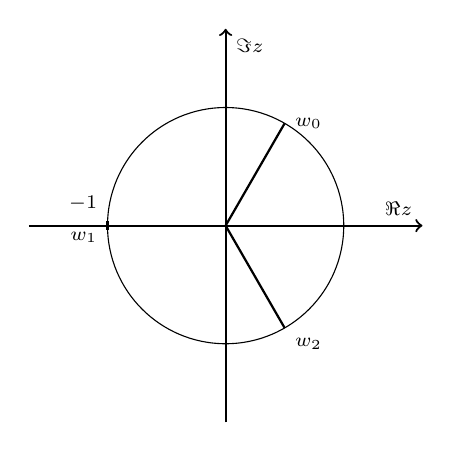
\begin{tikzpicture}[scale=0.5]
\begin{scope}[thick,font=\scriptsize]
\draw [->] (-5,0) -- (5,0) node [above left]  {$\Re z$};
\draw [->] (0,-5) -- (0,5) node [below right] {$\Im  z$};
\draw (-3,-3pt) -- (-3,3pt) node [above left] {$-1$} node [below left] {$w_1$};
\draw (0,0) -- (1.5, 2.6)  node [right] {$w_0$};
\draw (0,0) -- (1.5, -2.6) node [below right] {$w_2$};
\end{scope}
\path [draw=black,fill=none] (0,0) circle (3);
\end{tikzpicture}
\end{center}

\end{Examples}

\subsection{Решение квадратных уравнений с комплексными коэффициентами}

Пусть дано квадратное уравнение $az^2+bz+c=0$, где $a,\ b,\ c\in\mathbb{C}$ и 	$ a \neq 0$. Тогда имеем:
\begin{gather*}
    z^2+\frac{b}{a}z+\frac{c}{a} = 0\\
    z^2+2\frac{b}{2a}z+\frac{b^2}{4a^2}+\frac{c}{a}-\frac{b^2}{4a^2} = 0\\
    \left(z+\frac{b}{2a}\right)^2=\frac{b^2-4ac}{4a^2}\\
    z+\frac{b}{2a} \in \sqrt{\frac{b^2-4ac}{4a^2}}=\frac{\sqrt{b^2-4ac}}{2a}
\end{gather*}

То есть все решения --- это $z_1 = \cfrac{-b+d_1}{2a},\ z_2 = \cfrac{-b+d_2}{2a}$, где $\{d_1,d_2\} = \sqrt[2]{b^2-4ac}$. В частности, квадратное уравнение всегда имеет комплексный корень, а при $b^2-4ac\neq0$ два корня.

\begin{Theorem}[Основная теорема алгебры]
Всякий многочлен $P\left(z\right) = a_nz^n + a_{n-1}z^{n-1} + \ldots \hm{+} a_1z + a_0$ степени $n$, где $n \geqslant 1$, $a_n \neq 0$, и $a_0,\ldots,a_n \in \mathbb{C}$ имеет корень.
\end{Theorem}

\subsection{Векторные пространства над произвольным полем}

И снова вспомним, что такое векторное пространство:

\begin{itemize}
    \item некоторое множество $V$;
    \item есть операция сложения $V\times V\rightarrow V$;
    \item есть операция умножения на скаляр $F\times V\rightarrow V$;
    \item выполняются 8 аксиом.
\end{itemize}

Все основные понятия и результаты теории векторных пространств из прошлого полугодия можно перенести на случай пространства над произвольным полем $F$ без изменений.

\begin{Examples}
Пусть $V$ --- векторное пространство над полем из двух элементов, $\dim V = n$. Тогда $|V| = 2^n$. Действительно, каждое конечномерное пространство обладает базисом (в данном случае $e_1,\ldots,e_n$). Тогда $V = \{k_1e_1+k_2e_2+\ldots+k_ne_n\ |\ k_i\in F\}$. Но очень легко заметить, что всего таких линейных комбинаций $2^n$
\end{Examples}
